\section{中等质量区间}

在中等质量区间当中,夸克胶子等离子体热辐射所产生的双电子占据了主要部分。所以在这个质量区间的拟合当中只使用了\ref{eq:QGP_thermal}作为拟合方程。NA60实验也在\sNN = 17.3 GeV铟-铟对撞中对来源于夸克胶子等离子体热辐射的双轻子进行了测量,其测量得到的温度结果为205 $\rm{ \pm }$ 12 MeV\cite{Specht:2010xu}。STAR实验\sNN = 54.4 GeV, \sNN = 27 GeV 金-金对撞中在双电子谱的中等质量区间抽取结果如图\ref{fig:Hm_ExY_FMR_54GeV_27GeV_NA60_QGPfit_icent0}所示。这是首次在RHIC上通过测量双轻子谱的方式对夸克胶子等离子体的温度进行了测量。并且因为是通过双电子的方式对温度进行测量,可以有效的避免介质的流对最终温度测量结果的影响。在不同的中心度下的中等质量区间内的温度抽取结果见表\ref{T_fitting_result_IMR}。

可以看到STAR实验中\sNN = 54.4 GeV, \sNN = 27 GeV两者在中等质量区间所抽取得到的温度在误差范围内符合的很好。和NA60实验的结果相比,STAR实验的结果均高于其测量得到的205 $\rm{ \pm }$ 12 MeV的结果。如果和理论计算相比,三者的温度都要高于理论计算中得到的相变温度 $\rm{T_{pc} =154~ MeV}$\cite{HotQCD:2018pds}。这也证明了在这个区间双轻子主要来源于一个更高温的物质的态,即夸克胶子等离子体态。

\begin{figure}[htb]
    \begin{center}
    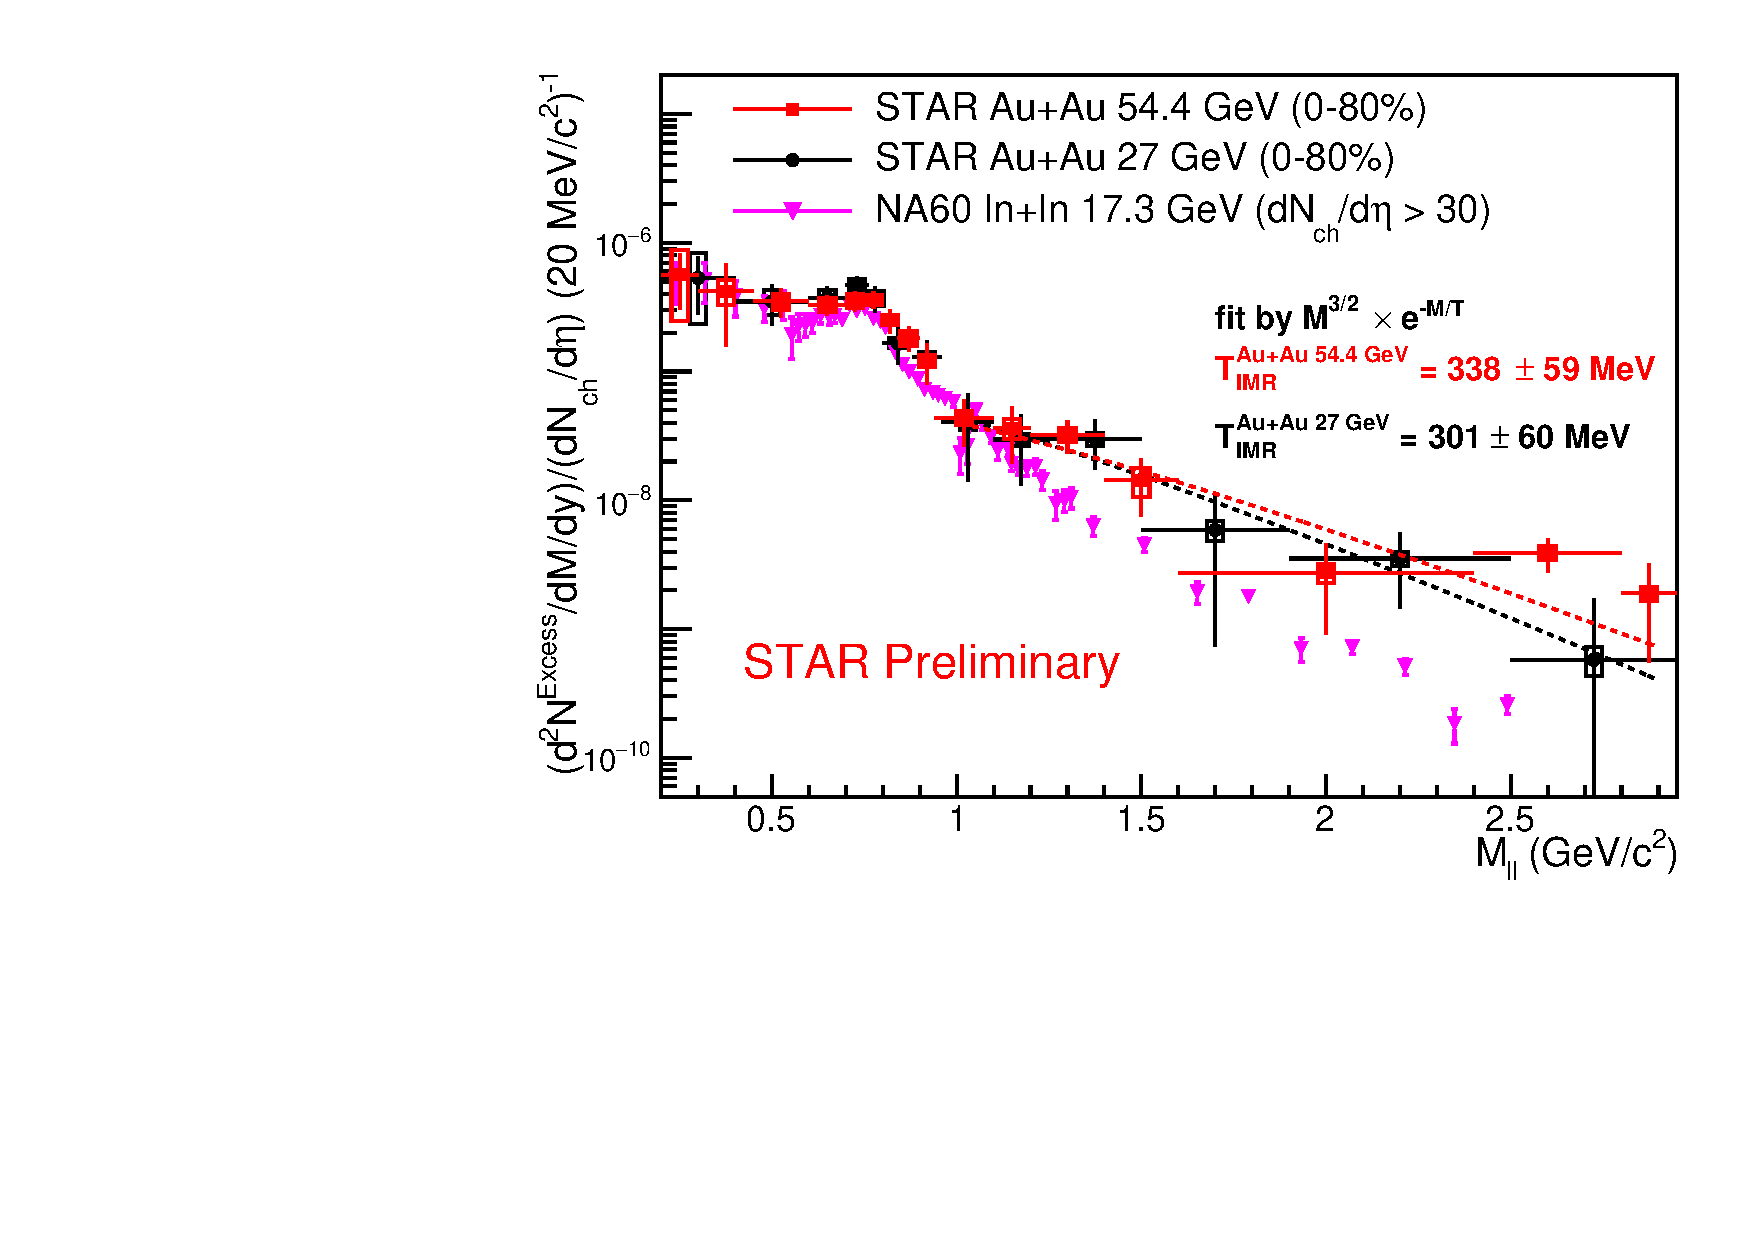
\includegraphics[width=0.75\textwidth,clip]{figures/Chapter4/Hm_ExY_FMR_54GeV_27GeV_NA60_QGPfit_icent0.pdf}
    \end{center}
    \caption[STAR实验中 \sNN = 54.4 GeV, \sNN = 27 GeV 金-金对撞以及NA60实验中\sNN = 17.3 GeV铟-铟对撞中双轻子额外产额比较示意图]{STAR实验中 \sNN = 54.4 GeV, \sNN = 27 GeV 金-金对撞以及NA60实验中\sNN = 17.3 GeV铟-铟对撞中双轻子额外产额比较示意图。在中等质量区间通过方程\ref{eq:QGP_thermal}拟合来抽取介质温度,STAR实验的抽取结果列在图中。}
    \label{fig:Hm_ExY_FMR_54GeV_27GeV_NA60_QGPfit_icent0}
\end{figure}

\begin{table}[h!]
    \centering
    \caption{54.4GeV金-金对撞中中等质量区间不同中心度通过拟合抽取得到的温度的结果}
    \label{tab:T_fitting_result_IMR}
    \begin{tabularx}{1\textwidth} {
    | >{\centering\arraybackslash}X |>{\centering\arraybackslash}X |>{\centering\arraybackslash}X |>{\centering\arraybackslash}X |>{\centering\arraybackslash}X | }
        \hline
        Centrality  & $T_{med}$ \\
        \hline
        0-80\%  & $338 \pm 58$ \\
        \hline
        0-10\%  & $371 \pm 123$ \\
        \hline
        10-40\% & $320 \pm 59$ \\
        \hline
        40-80\% & $336 \pm 55$ \\
        \hline
    \end{tabularx}
\end{table}